\documentclass[article]{report} % a4paper
% Some basic packages

\usepackage[utf8]{inputenc}
\usepackage[T1]{fontenc}
\usepackage{textcomp}
% Figure out whether you need this in English 
\usepackage[UKenglish]{babel}
\usepackage{url}
\usepackage{graphicx}
\usepackage{float}
\usepackage{booktabs}
\usepackage{enumitem}

% Don't indent paragraphs, leave some space between them
\usepackage{parskip}

% Hide page number when page is empty
\usepackage{emptypage}
\usepackage{subcaption}
\usepackage{multicol}
\usepackage{xcolor}

% Other font I sometimes use.
% \usepackage{cmbright}

% Math stuff
\usepackage{amsmath, amsfonts, mathtools, amsthm, amssymb}
% \usepackage{physics}
% Fancy script capitals
\usepackage{mathrsfs}
\usepackage{cancel}
% Bold math
\usepackage{bm}
% Some shortcuts
\newcommand\N{\ensuremath{\mathbb{N}}}
\newcommand\R{\ensuremath{\mathbb{R}}}
\newcommand\Z{\ensuremath{\mathbb{Z}}}
\renewcommand\O{\ensuremath{\emptyset}}
\newcommand\Q{\ensuremath{\mathbb{Q}}}
\newcommand\C{\ensuremath{\mathbb{C}}}
\newcommand\T{\ensuremath{\mathbb{T}}}
\newcommand\U{\ensuremath{\mathscr{U}}}
\newcommand\Y{\ensuremath{\mathscr{Y}}}
\newcommand\F{\ensuremath{\mathbb{F}}}

\newcommand{\norm}[1]{\left\lVert#1\right\rVert}
\let\newforall\forall
\renewcommand\forall{\;\newforall\;}
% Put x \to \infty below \lim
\let\svlim\lim\def\lim{\svlim\limits}

%Make implies and impliedby shorter
\let\implies\Rightarrow
\let\impliedby\Leftarrow
\let\iff\Leftrightarrow
\let\epsilon\varepsilon

% Add \contra symbol to denote contradiction
\usepackage{stmaryrd} % for \lightning
\newcommand\contra{\scalebox{1.5}{$\lightning$}}

% \let\phi\varphi

% Command for short corrections
% Usage: 1+1=\correct{3}{2}

\definecolor{correct}{HTML}{009900}
\newcommand\correct[2]{\ensuremath{\:}{\color{red}{#1}}\ensuremath{\to }{\color{correct}{#2}}\ensuremath{\:}}
\newcommand\green[1]{{\color{correct}{#1}}}

% horizontal rule
\newcommand\hr{
    \noindent\rule[0.5ex]{\linewidth}{0.5pt}
}

% hide parts
\newcommand\hide[1]{}

% si unitx
\usepackage{siunitx}
\sisetup{locale = FR}

% Environments
\makeatother
% For box around Definition, Theorem, \ldots
\usepackage{mdframed}
\mdfsetup{skipabove=1em,skipbelow=0em}
\theoremstyle{definition}
\newmdtheoremenv[nobreak=true]{consequence}{Consequence}
\newmdtheoremenv[nobreak=true]{theorem}{Theorem}
\newmdtheoremenv[nobreak=true]{lemma}{Lemma}
\newmdtheoremenv[nobreak=true]{definition}{Definition}
\newmdtheoremenv[nobreak=true]{prop}{Proposition}
\newmdtheoremenv[nobreak=true]{law}{Law}
\newmdtheoremenv[nobreak=true]{corollary}{Corollary}
\newmdtheoremenv{conclusion}{Conclusion}
\newmdtheoremenv{bonus}{Bonus}
\newtheorem*{notation}{Notation}
\newtheorem*{issue}{Issue}
\newtheorem*{terminology}{Terminology}
\newtheorem*{application}{Application}
\newtheorem*{example}{Example}
\newtheorem*{eg}{Example}
\newtheorem*{question}{Question}
\newtheorem*{previouslyseen}{As previously seen}
\newtheorem*{remark}{Remark}
\newtheorem*{problem}{Problem}
\newtheorem*{observe}{Observe}
\newtheorem*{property}{Property}
\newtheorem*{intuition}{Intuition}
\newtheorem*{fact}{Fact}
\newtheorem*{result}{Result}
\newtheorem*{punch}{Punchline}

% Fix some spacing
% http://tex.stackexchange.com/questions/22119/how-can-i-change-the-spacing-before-theorems-with-amsthm
\makeatletter
\def\thm@space@setup{%
  \thm@preskip=\parskip \thm@postskip=0pt
}

% \lecture starts a new lecture (les in dutch)
%
% Usage:
% \lecture{1}{di 12 feb 2019 16:00}{Inleiding}
%
% This adds a section heading with the number / title of the lecture and a
% margin paragraph with the date.

% I use \dateparts here to hide the year (2019). This way, I can easily parse
% the date of each lecture unambiguously while still having a human-friendly
% short format printed to the pdf.

\usepackage{xifthen}
\def\testdateparts#1{\dateparts#1\relax}
\def\dateparts#1 #2 #3 #4 #5\relax{
    \marginpar{\small\textsf{\mbox{#1 #2 #3 #5}}}
}

\def\@lecture{}%
\newcommand{\lecture}[3]{
    \ifthenelse{\isempty{#3}}{%
        \def\@lecture{Lecture #1}%
    }{%
        \def\@lecture{Lecture #1: #3}%
    }%
    \subsection*{\@lecture}
    \marginpar{\small\textsf{\mbox{#2}}}
}



% These are the fancy headers
\usepackage{fancyhdr}
\pagestyle{fancy}

% LE: left even
% RO: right odd
% CE, CO: center even, center odd
% My name for when I print my lecture notes to use for an open book exam.
% \fancyhead[LE,RO]{Joseph Grosso}

\fancyhead[RO,LE]{\@lecture} % Right odd,  Left even
\fancyhead[RE,LO]{}          % Right even, Left odd

\fancyfoot[RO,LE]{\thepage}  % Right odd,  Left even
\fancyfoot[RE,LO]{}          % Right even, Left odd
\fancyfoot[C]{\leftmark}     % Center

\makeatother




% Todonotes and inline notes in fancy boxes
\usepackage{todonotes}
\usepackage{tcolorbox}

% Make boxes breakable
\tcbuselibrary{breakable}

% Usage: 
% \begin{correction}
%     Lorem ipsum dolor sit amet, consetetur sadipscing elitr, sed diam nonumy eirmod
%     tempor invidunt ut labore et dolore magna aliquyam erat, sed diam voluptua. At
%     vero eos et accusam et justo duo dolores et ea rebum. Stet clita kasd gubergren,
%     no sea takimata sanctus est Lorem ipsum dolor sit amet.
% \end{correction}
\newenvironment{correction}{\begin{tcolorbox}[
    arc=0mm,
    colback=white,
    colframe=green!60!black,
    title=Correction,
    fonttitle=\sffamily,
    breakable
]}{\end{tcolorbox}}

% Note -- Same as 'correction' but color of box is different
\newenvironment{note}{\begin{tcolorbox}[
    arc=0mm,
    colback=white,
    colframe=white!60!black,
    title=Note,
    fonttitle=\sffamily,
    breakable
]}{\end{tcolorbox}}




% Figure support as explained in my blog post.
\usepackage{import}
\usepackage{xifthen}
\pdfminorversion=7
\usepackage{pdfpages}
\usepackage{transparent}
\newcommand{\incfig}[1]{%
    \def\svgwidth{\columnwidth}
    \import{./figures/}{#1.pdf_tex}
}

% Fix some stuff
% %http://tex.stackexchange.com/questions/76273/multiple-pdfs-with-page-group-included-in-a-single-page-warning
\pdfsuppresswarningpagegroup=1

% Remove leading zeroes from table of contents 
\renewcommand{\thesection}{\arabic{section}}

% My name
\author{Joseph Grosso}


\author{Joseph Grosso \and 
	Kyle Singer \and 
	Andrew Fryer \and
	Andrew Farley}
\usepackage{titling}

\DeclareMathOperator{\length}{length}
\DeclareMathOperator{\Aut}{Aut}
\DeclareMathOperator{\diam}{diam}
\DeclareMathOperator*{\res}{res}
\title{Team Carnation: \\ Power Generation }
\pretitle{%
  \begin{center}
  \LARGE
  
\includegraphics[width=4cm,height=8cm]{./figures/carnation.png}\\[\bigskipamount]
}
\posttitle{\end{center}}

\begin{document}
    \maketitle
    \tableofcontents

    \section{Introduction}
    Our challenge is to create an algorithm that acts as a single power grid for the entire province of Ontario. The program will address the energy needs of the province, taking into account the supply and demand of power from various sources. Our system addresses both the needs of the consumer (minimizing black/brownouts, minimizing price) and prioritizes green energy sources to limit environmental impact of the energy system. 

    \section{Considerations}
    Our group took into account many issues to create our algorithm, which will be outlined below.
    \subsection{Energy Cost}
    Our algorithm had to minimize the cost of the energy production, to ensure that the Hydro System would not be losing money. 
    \subsection{CO$_{2}$ Production} 
    The algorithm also had to take into account the price of using sources of carbon emissions, contributing to the global warming crisis.
    \subsection{Reliability}
    Our customers need to be able to rely on the power grid. Our algorithm has to ensure that customers will not experience blackouts, brownouts, or power cuts of any kind. 

    \section{Solution}
    \subsection{Algorithm}
    The heart of the algorithm is a priority queue, ranking the energy sources by their benefits according to our considerations. Using these, we were able to create score functions for each power source providing us with our priority queue which we could draw power in order from. 
    
    The score functions looked like this:
    \begin{align*}
	    \text{Green Score } &= \begin{cases}
		1 & \text{ if energy source } \in  \text{Solar, Wind, Hydro, Biofuel} \\
		0.8 & \text{ otherwise}
    	\end{cases} \\
		    \text{CO}_{2} \text{ Score} &= 1 - \left( \frac{\text{CO}_{2} \text{Emissions}\left( \text{source} \right) }{B \times MAX \left( CO_{2} \text{Emissions} \right) } \right) \\ % TODO: Replace B with an appropriate number we decide on 
		    \text{Cost Score} &= 1 - \left( \frac{\text{cost}\left( s \right) }{C \times  MAX \left( \text{cost} \right) } \right) \\
		    \text{Source Score } &=  \text{Green Score } + \text{CO}_{2} \text{ Score} + \text{Cost Score}
    .\end{align*}
    
    Because all power created by the Nuclear source had to be used, in our algorithm we used all Nuclear power first and then split up the remaining power demand according to our priority. To decide how we should change the amount of Nuclear power generated on each iteration, we used the following equation:
    \begin{align*}
	    \text{Movement\_Direction } &= \frac{t_{n + 1} }{t_{n}} - 1 \\
	    \text{Nuc. Source Change } &= \text{clamp} 
	    \left( \text{Movement\_Direction}  \times \text{Nuc. Source} + \text{Nuc. Source}, -0.01, 0.01 \right)  
    .\end{align*}

    where $t_{n}$ is the total energy usage as of one week ago, movement direction tells us the direction that the nuclear power generation will be moving in, and the clamp function caps the movement of the nuclear source at 1\%.

    \subsection{Implementation}
    We implemented our algorithm in Python, using the libraries Pandas and Numpy. We also used MatPlotLib to do visualizations of our data output. 

    \section{Conclusion}
    We implemented our code and found it to be successful. We were able to generate an algorithm which balances the CO$_{2}$ emissions of the energy generation with selling enough power to be profitable in every hour (approx. \$410,000 per hour). While our CO$_{2}$ emissions were higher than expected we should be able to improve the algorithm in the future. 

    \begin{figure}[htpb]
    	\centering
	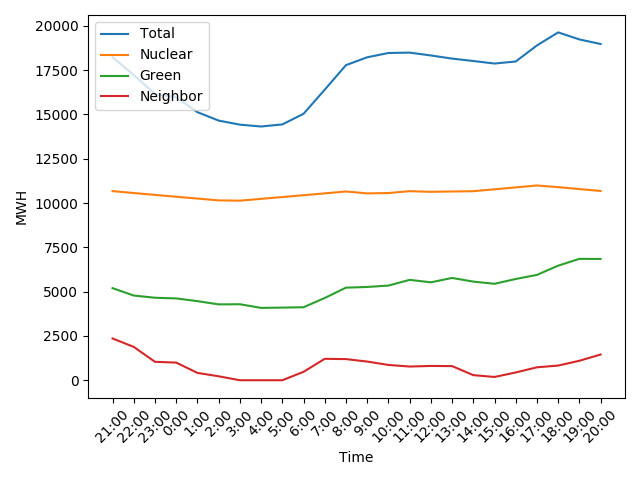
\includegraphics[width=0.8\textwidth]{figures/myplot.png}
    	\caption{Time vs. MWH generated by each energy source}
    	\label{fig:}
    \end{figure}
\end{document}
